\documentclass[]{article}
\usepackage{lmodern}
\usepackage{amssymb,amsmath}
\usepackage{ifxetex,ifluatex}
\usepackage{fixltx2e} % provides \textsubscript
\ifnum 0\ifxetex 1\fi\ifluatex 1\fi=0 % if pdftex
  \usepackage[T1]{fontenc}
  \usepackage[utf8]{inputenc}
\else % if luatex or xelatex
  \ifxetex
    \usepackage{mathspec}
  \else
    \usepackage{fontspec}
  \fi
  \defaultfontfeatures{Ligatures=TeX,Scale=MatchLowercase}
\fi
% use upquote if available, for straight quotes in verbatim environments
\IfFileExists{upquote.sty}{\usepackage{upquote}}{}
% use microtype if available
\IfFileExists{microtype.sty}{%
\usepackage{microtype}
\UseMicrotypeSet[protrusion]{basicmath} % disable protrusion for tt fonts
}{}
\usepackage[margin=1in]{geometry}
\usepackage{hyperref}
\hypersetup{unicode=true,
            pdftitle={Simulation of PCB with resampling},
            pdfauthor={Xuelong Wang},
            pdfborder={0 0 0},
            breaklinks=true}
\urlstyle{same}  % don't use monospace font for urls
\usepackage{graphicx,grffile}
\makeatletter
\def\maxwidth{\ifdim\Gin@nat@width>\linewidth\linewidth\else\Gin@nat@width\fi}
\def\maxheight{\ifdim\Gin@nat@height>\textheight\textheight\else\Gin@nat@height\fi}
\makeatother
% Scale images if necessary, so that they will not overflow the page
% margins by default, and it is still possible to overwrite the defaults
% using explicit options in \includegraphics[width, height, ...]{}
\setkeys{Gin}{width=\maxwidth,height=\maxheight,keepaspectratio}
\IfFileExists{parskip.sty}{%
\usepackage{parskip}
}{% else
\setlength{\parindent}{0pt}
\setlength{\parskip}{6pt plus 2pt minus 1pt}
}
\setlength{\emergencystretch}{3em}  % prevent overfull lines
\providecommand{\tightlist}{%
  \setlength{\itemsep}{0pt}\setlength{\parskip}{0pt}}
\setcounter{secnumdepth}{5}
% Redefines (sub)paragraphs to behave more like sections
\ifx\paragraph\undefined\else
\let\oldparagraph\paragraph
\renewcommand{\paragraph}[1]{\oldparagraph{#1}\mbox{}}
\fi
\ifx\subparagraph\undefined\else
\let\oldsubparagraph\subparagraph
\renewcommand{\subparagraph}[1]{\oldsubparagraph{#1}\mbox{}}
\fi

%%% Use protect on footnotes to avoid problems with footnotes in titles
\let\rmarkdownfootnote\footnote%
\def\footnote{\protect\rmarkdownfootnote}

%%% Change title format to be more compact
\usepackage{titling}

% Create subtitle command for use in maketitle
\newcommand{\subtitle}[1]{
  \posttitle{
    \begin{center}\large#1\end{center}
    }
}

\setlength{\droptitle}{-2em}

  \title{Simulation of PCB with resampling}
    \pretitle{\vspace{\droptitle}\centering\huge}
  \posttitle{\par}
    \author{Xuelong Wang}
    \preauthor{\centering\large\emph}
  \postauthor{\par}
      \predate{\centering\large\emph}
  \postdate{\par}
    \date{2018-09-07}

\usepackage{float,amsmath, bbm, siunitx, bm}
\floatplacement{figure}{H}
\newcommand{\indep}{\rotatebox[origin=c]{90}{$\models$}}

\begin{document}
\maketitle

{
\setcounter{tocdepth}{2}
\tableofcontents
}
\section{Decorrelation using Graphical Lasso (glasso) and
motivation}\label{decorrelation-using-graphical-lasso-glasso-and-motivation}

Based on the previous simulation results, we found that the variance
estimator of proposed method is not very stable, means variance of the
estimator is large when the sample proportion is small. Thus, One
possible reason for that is the decorrelation procedure of the proposed
method is not that accurate. It uses the SVD method to find the inverse
covariance matrix, which could be too closed to the sample date to
capture the true structure of the covariance matrix. Therefore, we want
to try the glasso method which add penalty to the estimated inverse
covariance matrix if it's in favor of the sample data.

\subsection{Main Idea of glasso}\label{main-idea-of-glasso}

For the N multivariate normal observations of dimension p, with mean
\(\mu\) and covaraince \(\Sigma\).

To estimate the precision matrix, we could maximize the penalized
log-likelihood,

\[
  \log{|\Theta|} - tr(S\Theta) - \rho||\Theta||_1,
\]

where

\begin{itemize}
\tightlist
\item
  \(\Theta = \Sigma^{-1}\),\\
\item
  \(||\cdot||_1\) is for \(L_1\) norm - sum of all the absolute values
  of each elements of \(\Theta\),\\
\item
  \(S\) is the empirical covariance matrix.
\end{itemize}

Note: as other lasso method, the key assumption of glasso is the
sparsity of the covariance matrix \(\Sigma\)

\section{Simulation result}\label{simulation-result}

\subsection{Simulation result of the fixed
fixed}\label{simulation-result-of-the-fixed-fixed}

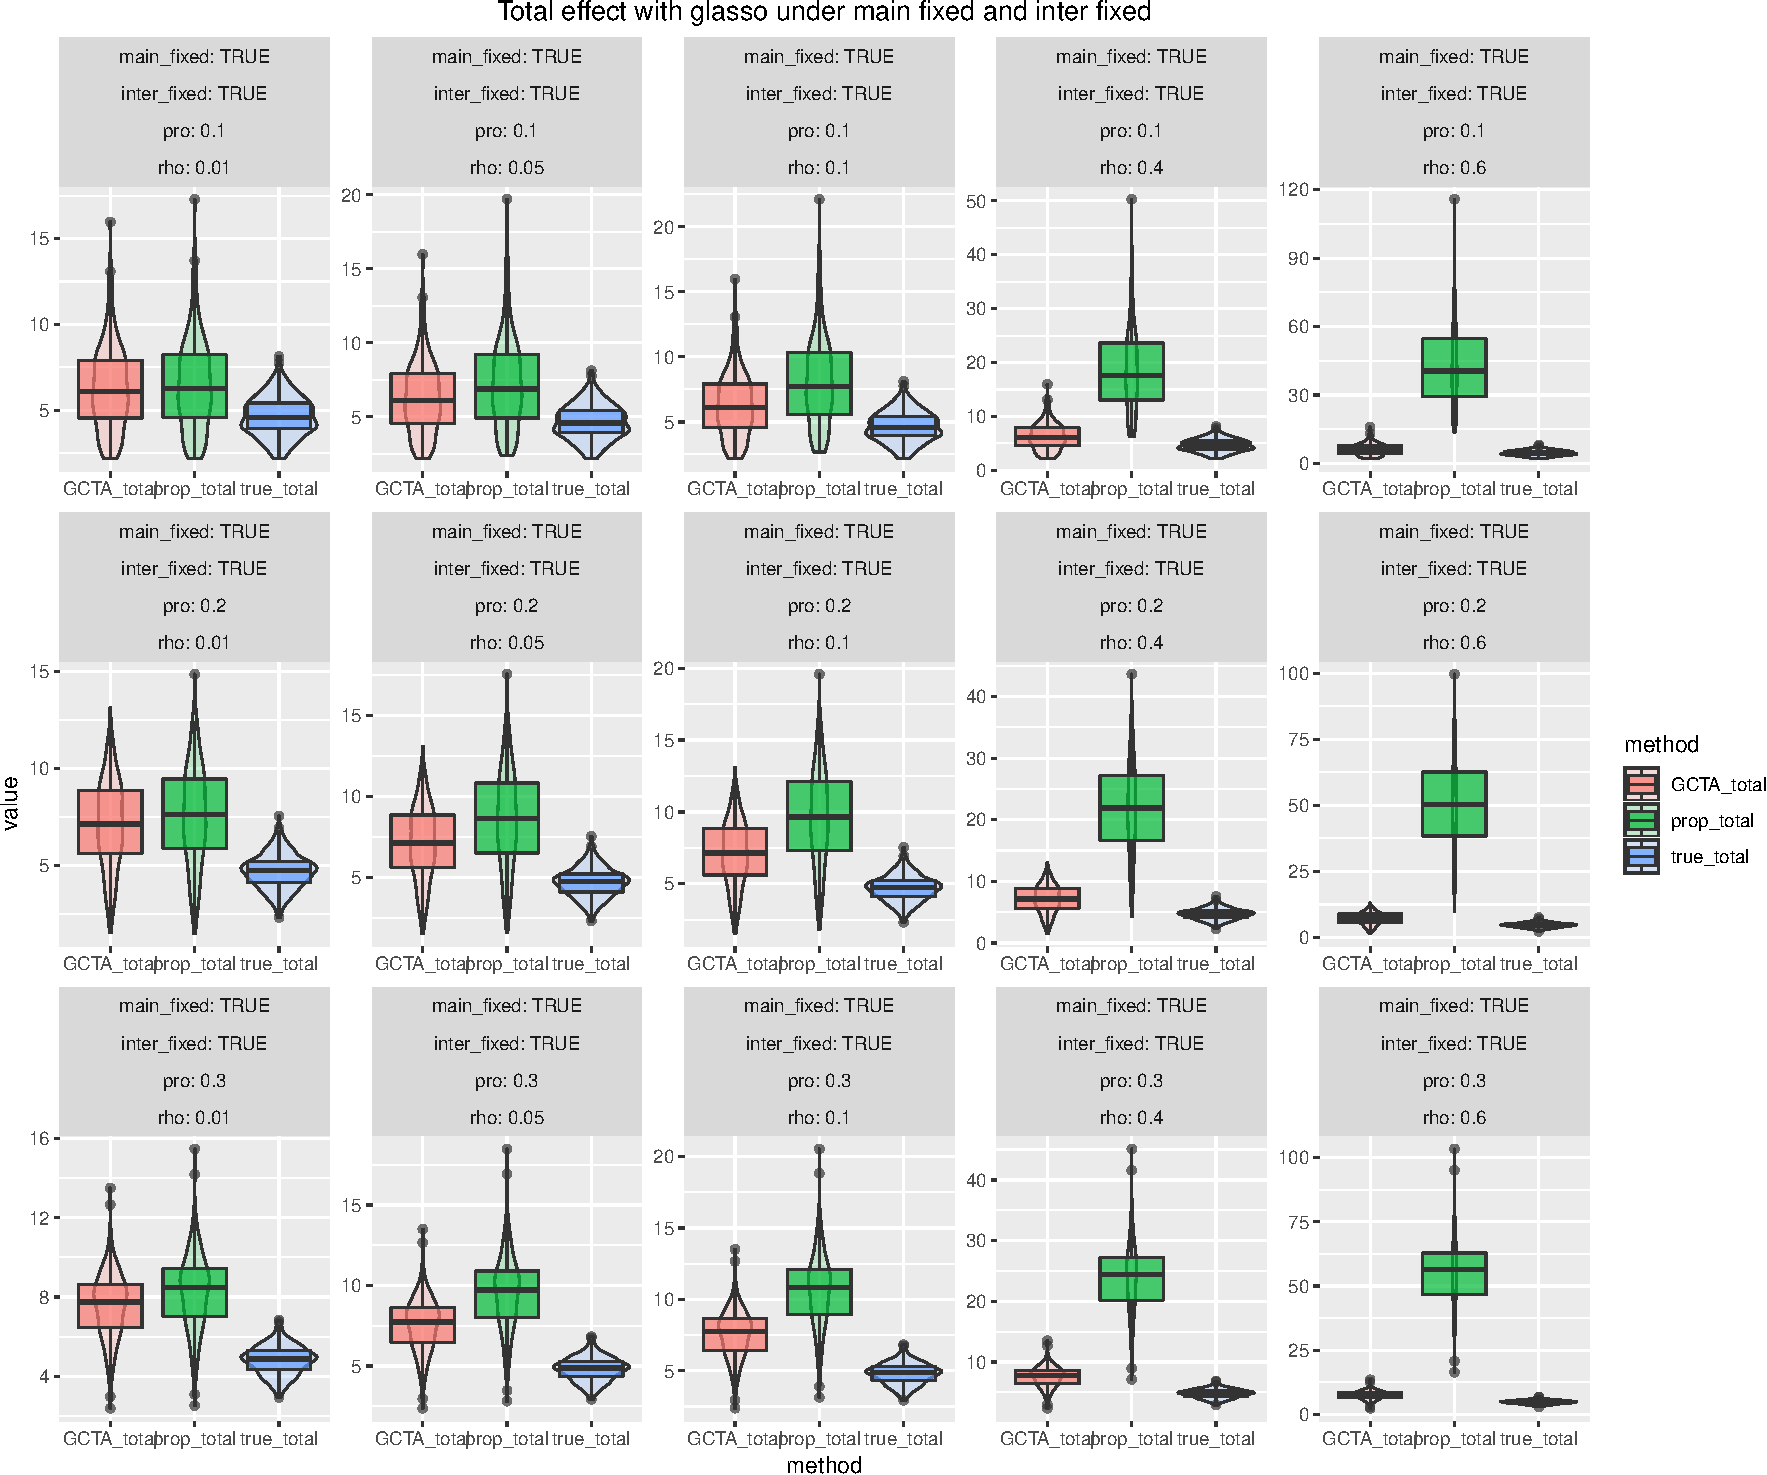
\includegraphics{Simulation_report_glasso_files/figure-latex/fixed fixed total glasso-1.pdf}
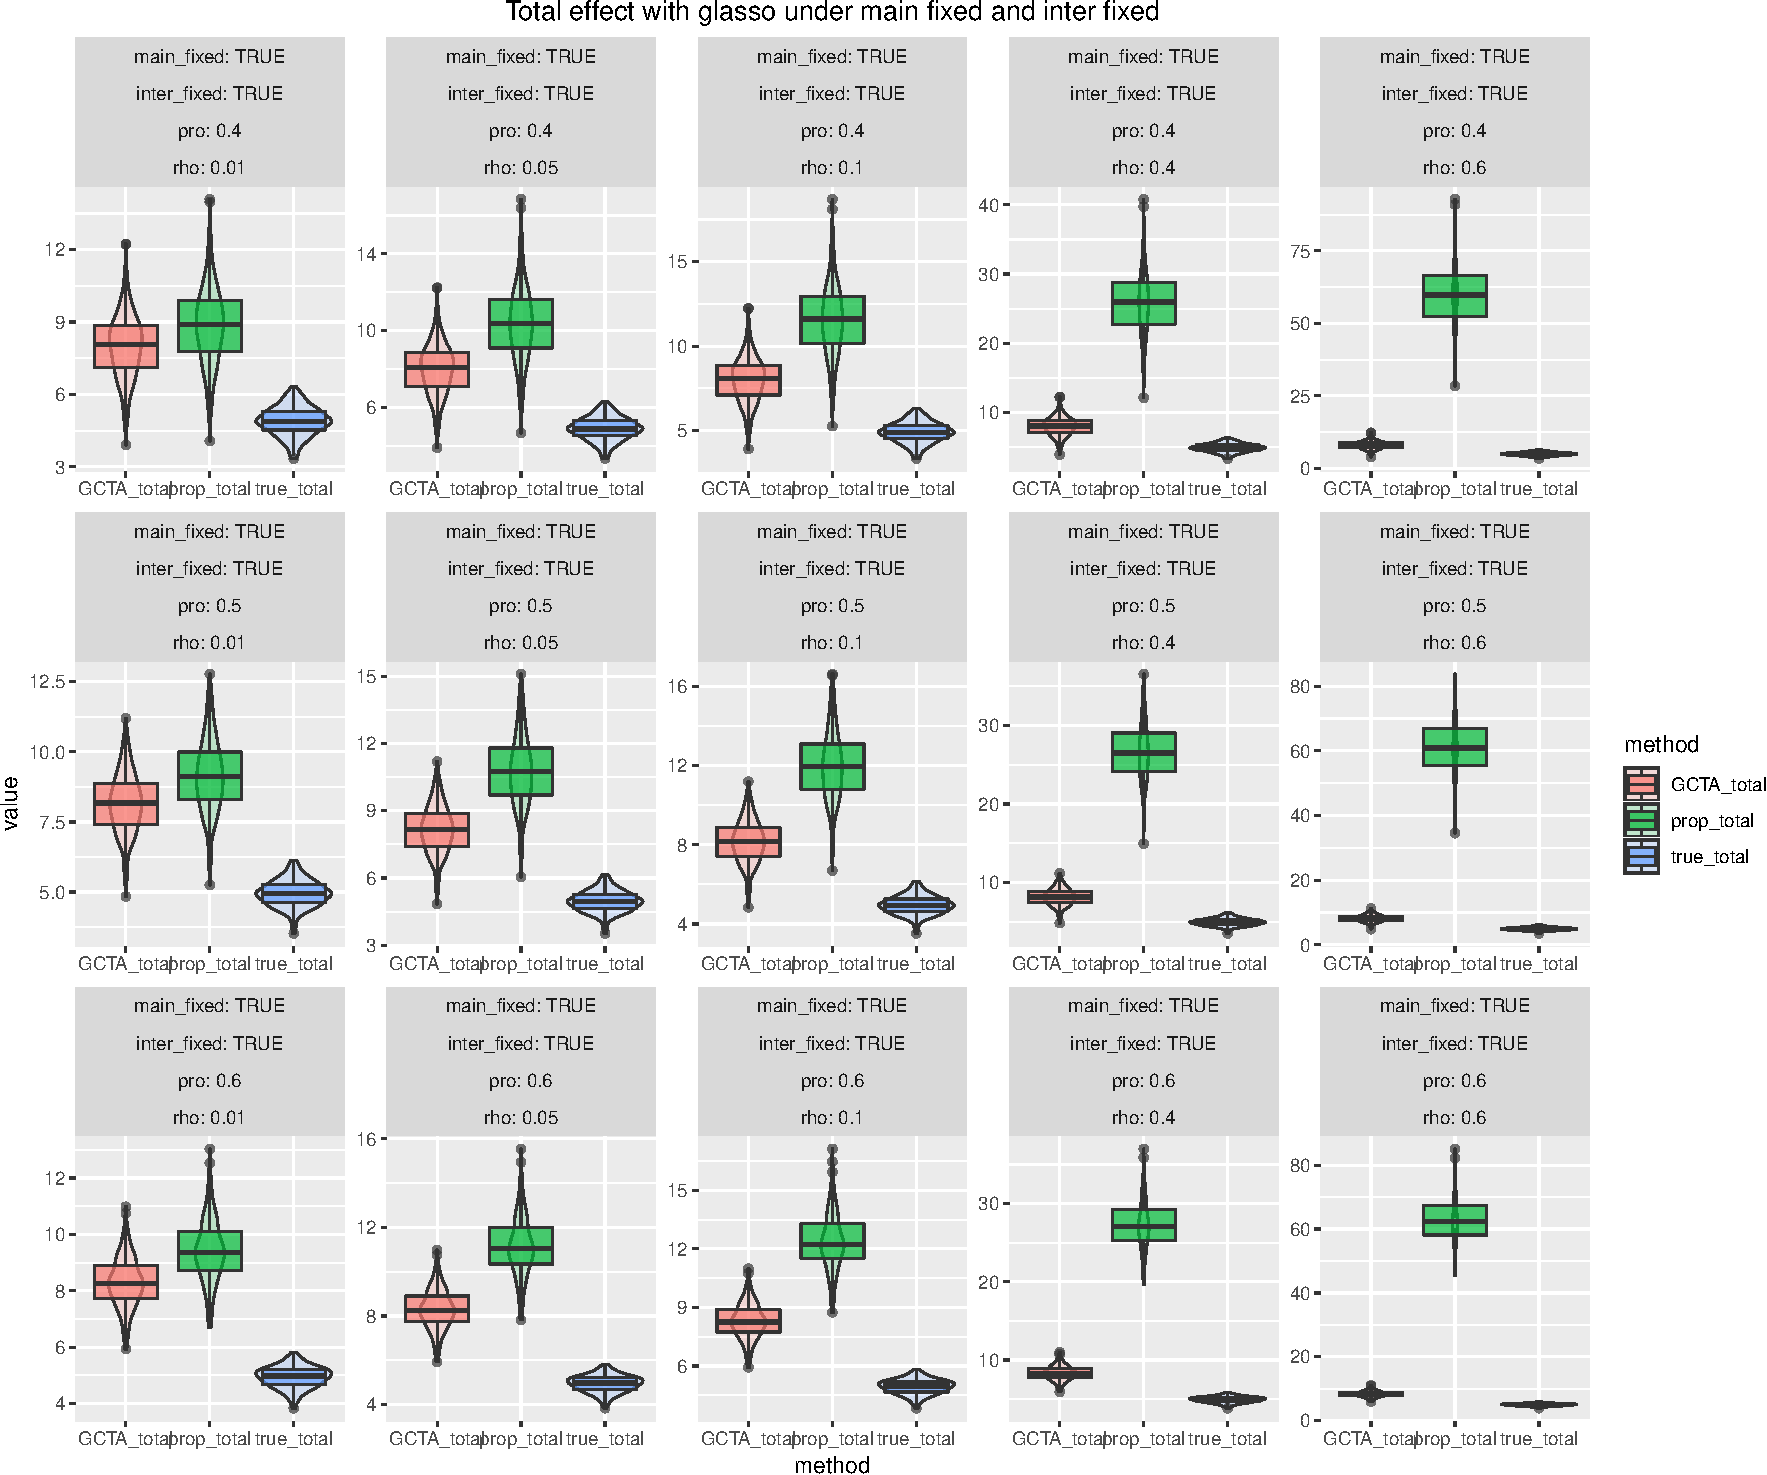
\includegraphics{Simulation_report_glasso_files/figure-latex/fixed fixed total glasso-2.pdf}
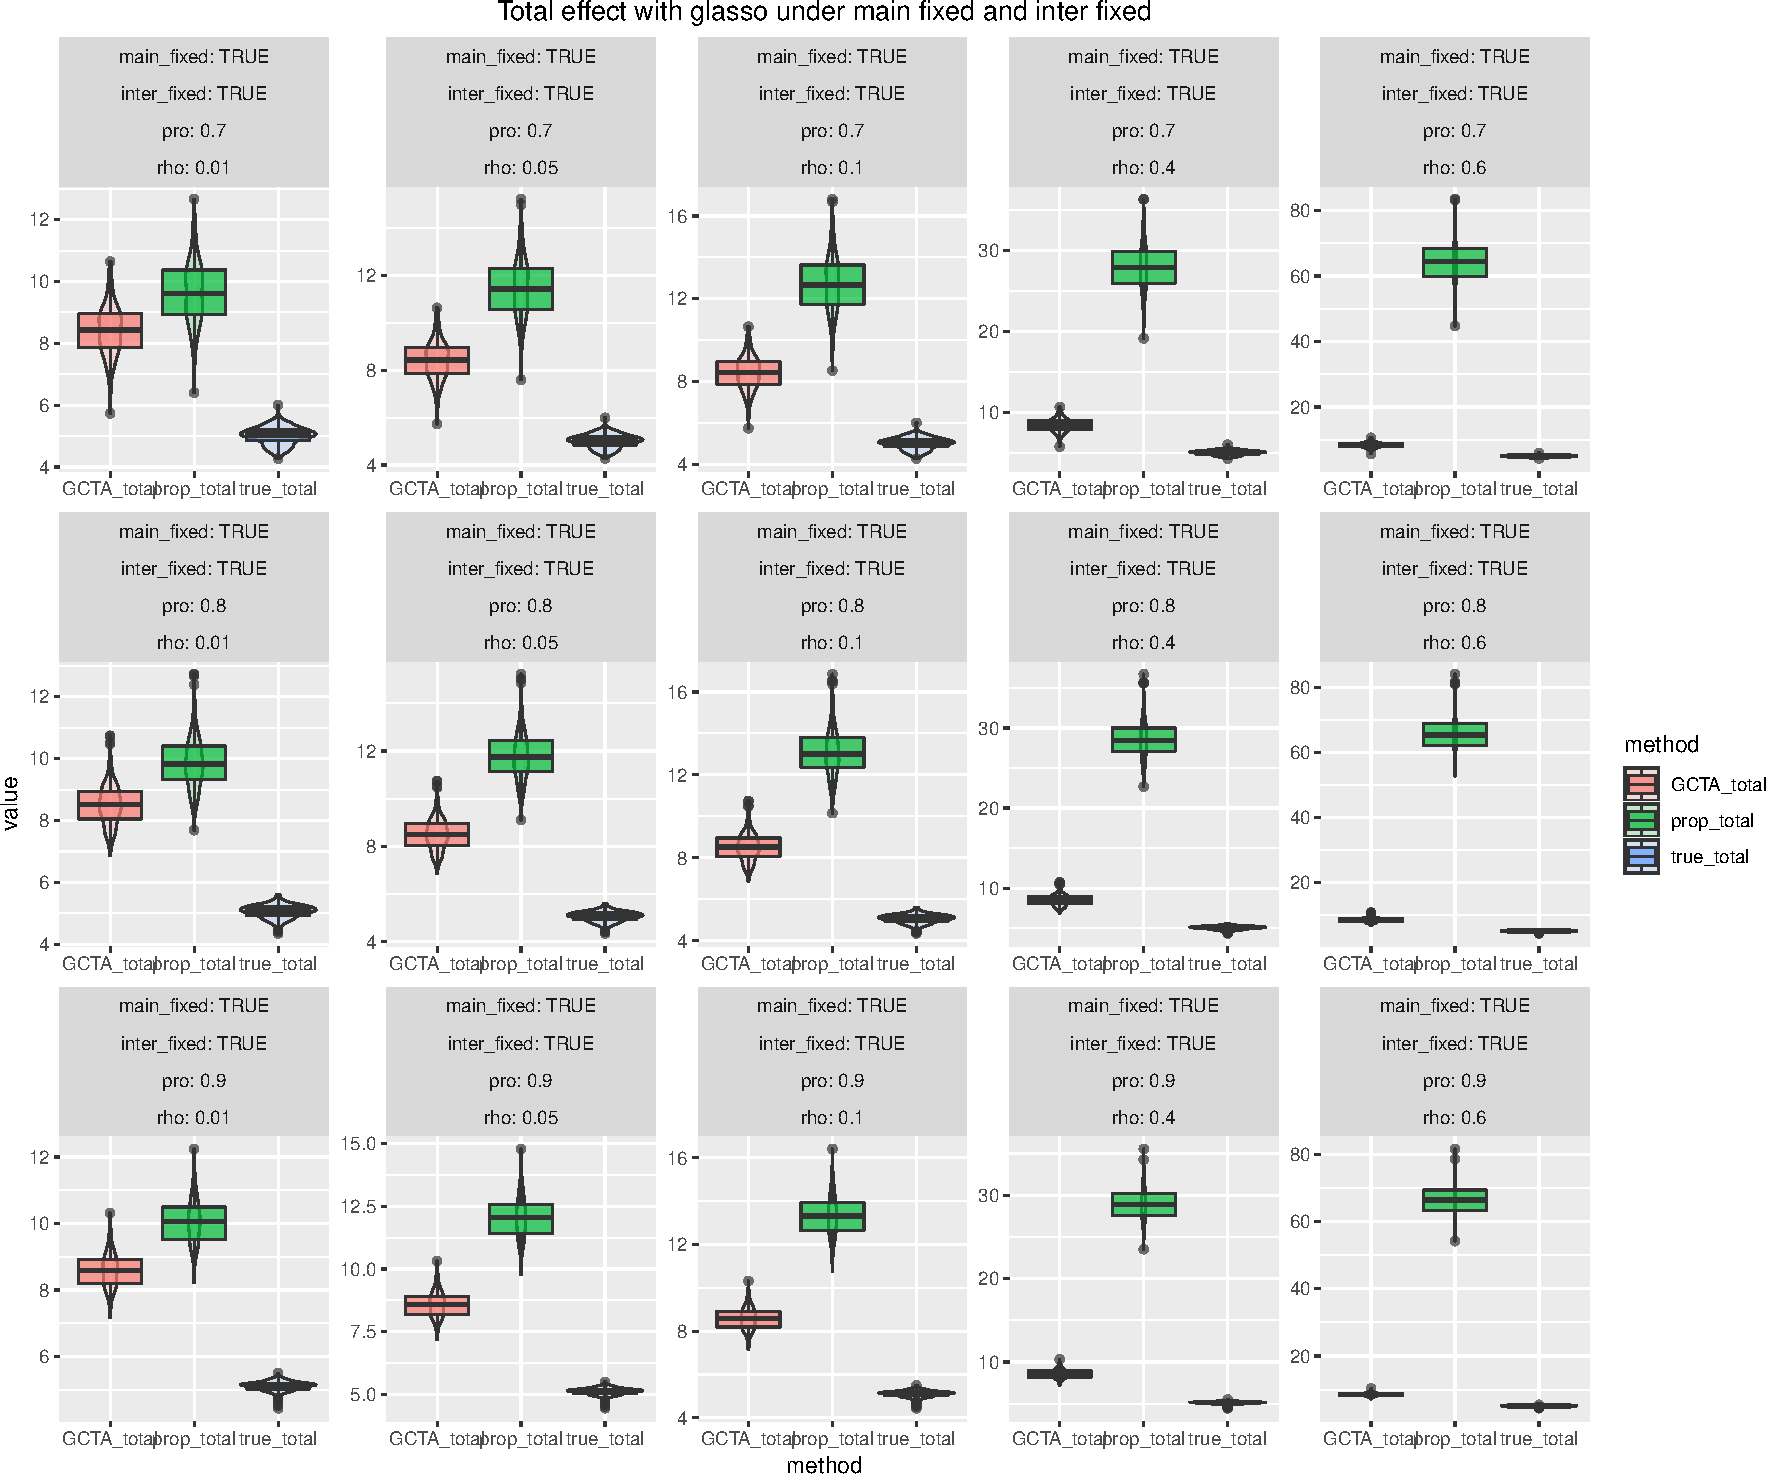
\includegraphics{Simulation_report_glasso_files/figure-latex/fixed fixed total glasso-3.pdf}

\section{Conclusion}\label{conclusion}

\section{Further work}\label{further-work}


\end{document}
